\documentclass[14pt]{article}
\usepackage[margin=1in, a4paper]{geometry}

\title{Discussion of Projects offered in the IITBombayX Cloud and Big Data group}
\author{Arinjoy Basak}

 \ifx\pdftexversion\undefined
 \usepackage[dvips]{graphicx}
 \else
 
 \usepackage[pdftex]{graphicx}
 \DeclareGraphicsRule{*}{mps}{*}{}
 \fi
\usepackage{url}
\usepackage{chapterbib}
\usepackage{hyperref}
\usepackage{lscape}
\usepackage{longtable}
\usepackage{float}
\usepackage{url}
\usepackage{multicol}
\usepackage{color}
\usepackage{amsmath}

\usepackage{fancyhdr}
\pagestyle{fancy}
\lhead{\leftmark}
\rhead{}
\lfoot{Arinjoy Basak	}
\cfoot{\today}
\rfoot{\thepage}

\renewcommand{\bibname}{References}

\setcounter{secnumdepth}{4}
\setcounter{tocdepth}{4}

\begin{document}

\begin{titlepage}
 \begin{center}
\Huge
\textbf{Discussion of Projects offered in the IITBombayX Cloud and Big Data group} \\
\vfill
\LARGE
\textbf{Arinjoy Basak}\\
\texttt{3rd Year B.E. Computer Science and technology, IIEST Shibpur, Howrah, West Bengal}\\
\vfill
\Large
Last Updated: \today
\end{center}
\end{titlepage}

%\pagebreak \textcolor{white}{text} \pagebreak
%\thispagestyle{empty}

\pagebreak
\setcounter{page}{1}
\pagenumbering{roman}

%\listoffigures ------ To add later for figures

%\pagebreak

%\listoftables ------- To add later for tables

%\pagebreak

\tableofcontents

\pagebreak

\setcounter{page}{1}
\pagenumbering{arabic}


\section{Introduction to the IITBombayX MOOC platform}

The IITBombayX platform is a Massively Open Online Course (MOOC) platform developed by maintained by the professors, professionals and students at IIT Bombay, with the sole aim of providing the benefits of extended online education to Indian learners, along with providing training workshops for the teachers (under the T10KT workshop programme). It was launched on	 the 66th Republic Day, 2015, and provided three courses in the beginning:\cite{IITBombayX}

\begin{itemize}
 \item Introduction to Computer Programming, by Prof. Deepak B Phatak and Prof. Supratik Chakraborty; Dept of Computer Science and Engineering;
 \item Thermodynamics by Prof. U. N. Gaitonde, Prof. U. V. Bhandarkar, and Prof. M. D. Atrey; Dept of Mechanical Engineering; 
 \item Signals and Systems by Prof. Vikram Gadre, Dept of Electrical Engineering.
\end{itemize}

\section{The OPENedX platform}

The IITBombayX MOOC platform is built on the OPENedX web-based platform \cite{OPENedXofficialarch}, whose server-side code is written primarily in Python, with Mako templates \cite{Mako} and Django for the web-application framework \cite{Django}. The code for the browser side is written in JavaScript and mostly CoffeeScript, with the conversion of CoffeeScript code to JavaScript in progress, particularly the moving of the codebase to the Backbone.js framework. Together with these, Open EdX uses the Sass and Bourbon framework for the CSS code.

A diagram of the OpenEdX platform, together with all of its components and pipelines is as follows:

\begin{figure}[hb]
 \centering
 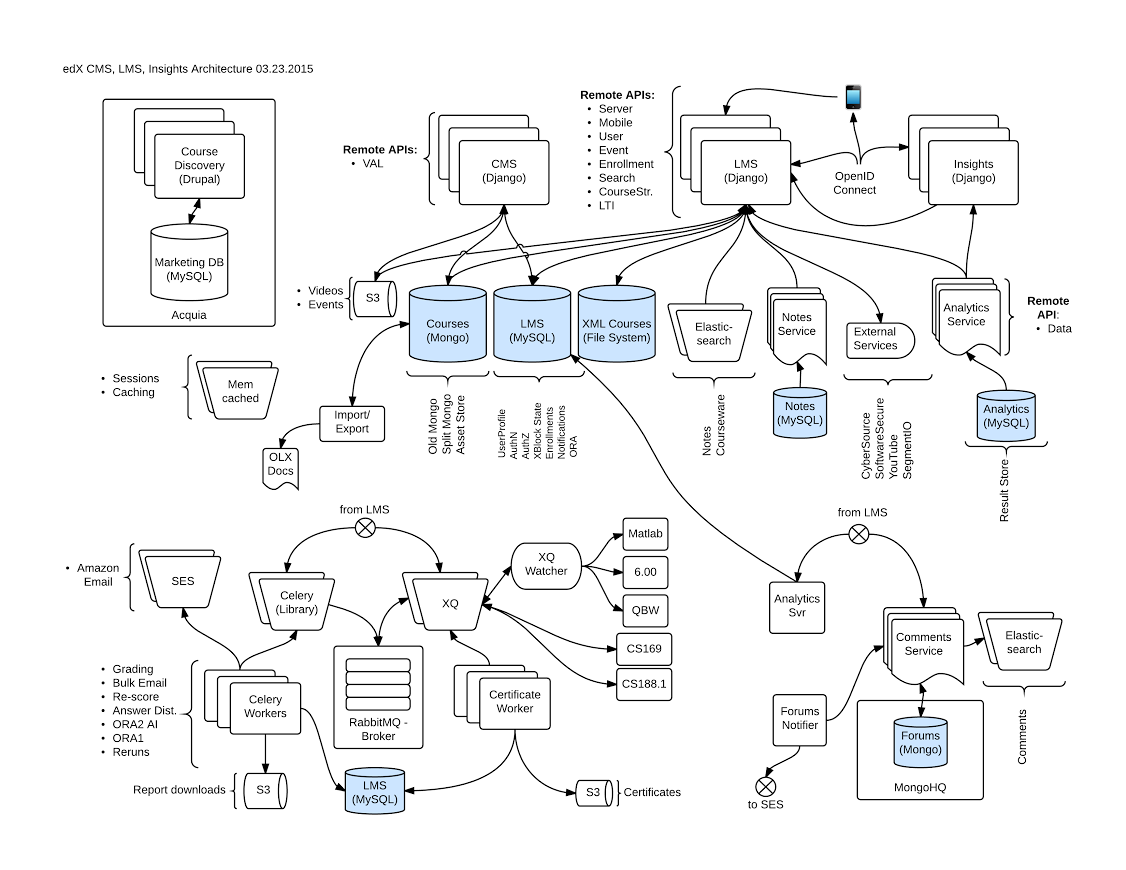
\includegraphics[width=12cm]{./edX_architecture_CMS_LMS_0.png}
 \caption{Open EdX components and pipelines, connecting the CMS (Course management System), LMS (Learning Management System) and the InSight Analytics System, together with the various services of the platform \label{fig:Image1}}
\end{figure}

\pagebreak

\section{The projects under the Cloud and Big data group}
The projects offered this year to the interns participating in the Summer Internship 2015 are as follows:

\begin{itemize}

\item 	Study and Integration of edX Insight
\item	Study of OpenStack cloud implementation
\item	Performance issues in IITBombayX Cloud
\item	Data Replication
\item	Exchange of data between Moodle and IITBombayX

\end{itemize}

\subsection{Study and Integration of edX Insight}

\subsubsection{What is edX Insight?}

InSight is a BI (business Intelligence) platform that was built by edX for the purpose of communicating the details of the courses, and analytical data concerning the student activity on the various courses to the administrators and course instructors. The primary aim of this platform is not only to monitor the student performances and validation of the choices made in designing the course, but also allows the designers to re-think the choices, and improve the course in its different aspects for creating a better experience for the students.

A BI platform, as defined by Gartner \cite{WhatIsBIPlatform}, provides a number of functionalities and services on a software platform. These can be primarily categorized into :

\begin{itemize}

\item Integration : This includes uniformity across the components used by the BI tools in terms of security, metadata and so on, sharing the same look and feel, together with providing a robust ways to access the data; as well as providing a development tools for programmers and a visual environment together, and the necessary APIs for integrating into the business process or other applications; and finally, the capability for BI users to share and discuss information and perform managerial tasks via multiple techniques.

\item Information Delivery : These include the functions of creating informative and concise parametrized reports from the, as well as provide web-based interactive methods for providing important information. Users mus also be able to ask and get answers regarding their own queries, and allow the searching of structured and unstructured data by mapping them to classification structures of dimensions and measures.

\item Analysis : The analysis capabilities include the OLAP capabilities of the data warehouses to allow users to access the data through drill-down processes of increasing details. Also, it provides interactive visual displays to express numerous aspects of data, with the future aim of providing improved visual representation workflow to stakeholders. It allows advanced mathematical techniques for classifying categorical variables and estimating continuous variables, with an aim to acheiving reliable predictions and allowing mining of interesting knowledge from the data; as well as provide metrics for measuring the performances and mapping them to the process of meeting strategic objectives.

\end{itemize}

\subsubsection{Why edX InSight?}

The study by Ma, Han, Yang and Chen \cite{ma2015examining} analyses the impact of an instructor on a student's engagement in an online learning environment, by building an interaction activity model for the teaching and learning process to track how a teacher's course preparation affects the different aspects of the students' engagement in the course, and how they are related to another. One of the key factors that was considered in this study was that it was not the student that was considered as the unit of study, but rather it was the course that was the unit of analysis; and in particular,the study used a learning analytics approach towards studying the problem, in which field, there have been few studies involving big data analysis in the online environment. It was showed that learning data analytics could be used to capture authentic, timely and objective evidence regarding online learning behaviour, with a focus towards college level online learning environments. The study was carried out on the THEOL Learning Management System, used in over four hundred universities and colleges in China.

A number variables were considered for study, among which several latent variables were clubbed together to create single variables for the hypotheses, which had six research hypotheses and five hypotheses for understanding the relations among the three dimensions of student engagement. The results of the study stated that the preparation activtities of the teacher/instructor is positively related to the student's viewing activities, and the guidance and assistance on the part of the instructor has a positive effect on the student being able to complete a learning task. This is also supported by the various  other studies conducted previously, and cited in the study, such as \cite{Morris2005221} and \cite{falakmasir2010using}. Thus, the need for data analytics is absolutely necessary for moving edX courses forward, and we need a platform to achieve the same. That is where edX Insight comes in.

\subsubsection{How does Insight work?}

The edX data analytics pipeline architecture is as shown (See \ref{fig:Image2}).

\begin{figure}[]
 \centering
 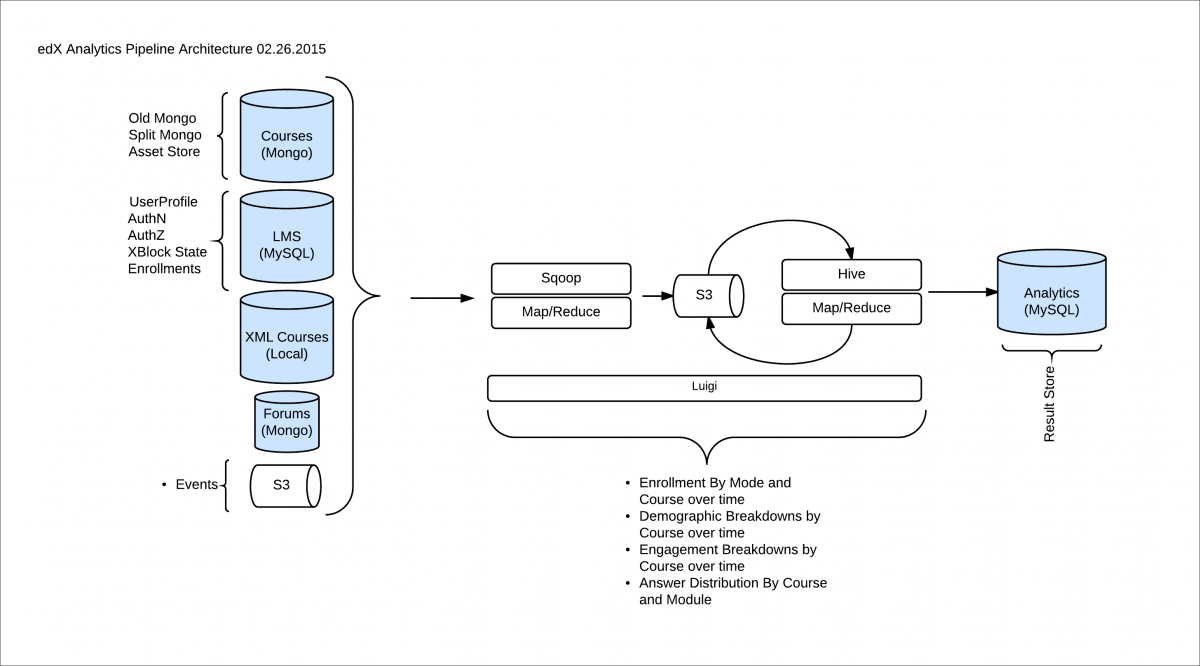
\includegraphics[width=12cm]{./edX_Architecture_Analytics.png}
 \caption{Open EdX Analytics pipelines \label{fig:Image2}}
\end{figure}

Insights is essentially a Django application that allows instructors and administrators to know about their students with respect to not oly course activity, but also demographic distributions, location based distributions, and educational qualifications, as we see later. The unstructured data in the form of events are stored in Amazon S3 as JSON objects, while the processed data is then stored in MySQL. Insight uses MySQL 5.1 for its purpose. The data is then transferred to Insights via a REST API.

edX Insights provides access to various graphs, metrics and reports for analysing the student behaviour and activity in different aspects, such as : How many students are enrolled in a course? Or, How are the student engaged with the course content - how are they performing, and how regularly are they accessing the course contents? It also covers the submissions made by the students in response to the questions posted on the course, based on both the grades received for the problems, as well as how the students are facing the questions and problems that do not add to their grades. There are also other analytical functions such as those for determining enrolment geography, which provides metrics for determining the countries of the students involved in the courses.

The methods used for computations of the various metrics can be found here \cite{edXInsightsCompRef}. Each of the computations are performed at a certain time, depending on the computation - even the metrics that are computed for reports available in the Instructor Dashboard occur at different times. Obviously, only the users enrolled for a course are included in the computations for that course - but this also means that the staff members, moderators and testers are also included in the computation., however, the activations of user accounts is not considered.

The functions provided by edX Insights are covered as follows \cite{edXInsights}:

\begin{itemize}

\item Course enrollment data is provided by Insight in the various forms, such as the daily student enrollment chart, enrollment metric, and enrollment over time metric. The daily student enrollment chart, for example, uses circles to depict periods of high student enrollment (in the form of spikes). The charts cover the educational programs such as honor certificate programs, verified certificate programs, and professional education programs. The number of enrolled students is computed everyday, together with updating the Enrollment Activty page on Insights.

\item Another important aspect of courses that needs to be monitored is the activity of the students in the courses, and how many of the students are actually active in the course. These include measures such as the weekly engagement charts, which measure the activty of the students over a one week period in terms of the completion of course activities, playing of videos and submission of answers to a problem. And then of course, there is the content engagement breakdown report, which is essentially a csv available for review or download, containing all the data collected on the course activity. The Engagement computation data are updated once a week,  usually on Mondays, while the computations themselves are made on Sunday. While the 'Active students' metric includes all activities, there are also specialized metrics which cover special topics such as watching of videos, and submission of problem solutions. As for ungraded answers, Insight allows the administrators to view the answers which are correct, and then allows veiwing of the actual answers that are received.

\item edX Insights also covers demographic data analysis of the students enrolled in a particular course, edX requires the students to provide data about themselves, and then analytics can be performed on the students data based on age bands and educational backgrounds (namely, the highest level of education completed), as well as gender.

\item Locations of the students are updated everyday, and so are the location based analytic functions and reports, which is particularly used in enrolment geography.

\item In addition, we have data on graded and ungraded contents, which are used to analyse how the students are answering the questions and what they find difficult, and whether they at all attempt the problems that do not add to the grades, and how they answer them. For answer submissions, the data is available in the form of the responses submitted (in the form of tags, internally). The computations for this data are updated on a a daily basis. 

\end{itemize}

\subsubsection{Application in edX}

This project requires us to study the edX Insight platform and its functioning, and then ultimately customize it and extend it for a final integration with IITBombayX. Particularly, this project will focus on extending the Insight platform with features especially suited to the Indian education environment.

\subsection{Study of OpenStack cloud implementation}

\subsection{What is OpenStack?}

OpenStack \cite{Openstack} provides software solutions for the pooling of large amounts of comupting, storage and networking resources thoughout a data center. The main mission behind the OpenStack project is to create a all-permeating Open Source Cloud Computing platform which can be used by private and and public clouds, regardless of the size, by being simple to implement and massively scalable. OpenStack is open source, openly designed and openly developed by an active community.

\subsubsection{How does OpenStack function?}

The OpenStack architecture can described using the following diagram:

 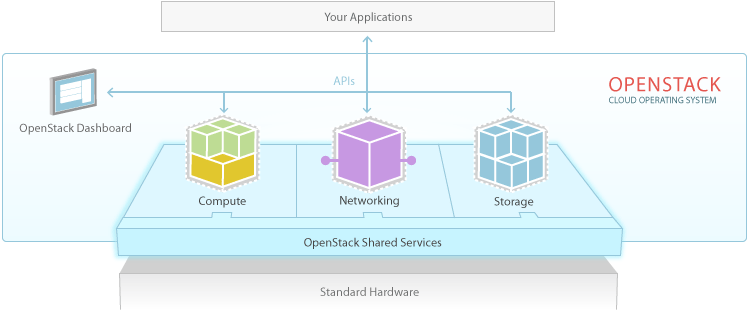
\includegraphics[width=12cm]{./openstack-software-diagram.png}

\begin{itemize}

\item OpenStack Compute \cite{OpenstackCompute} : The OpenStack cloud operating system allows the enterprises and software providers to provide computing resources to the customers on demand, when required. this is acheived by provisioning and managing of large virtual machines, which means that huge numbers of virtual machines are provided as and when required to fulfil the computing requirements of the customers. The resources are can be accessed by the APIs used by developers for building web applications and and web interfaces for administrators and users. Some of the popular roles played by OpenStack Compute include the roles in service providers providing IaaS services, or processing of big data.

\item OpenStack Storage \cite{OpenstackStorage} : OpenStack supports both Object and Block storage, meeting with variable performance and price criteria for organisations. An API accessible distributed platform is provided, which can be readily integrated into applications or used for simple data backup and similar tasks. For Object storage, OpenStack provides redundant, horizontally scalable object storage through clusters of servers capable of storing petabytes of data. Block storage is used for block level storage devices for use with OpenStack compute instances. This system allows the creation, attaxchment and detachment of blocks devices to servers, and the fact that they are ntegrated into the Dashboard and Compute allows Cloud users to handle their own storage requirements.

\item OpenStack Networking \cite{OpenstackNW} : Traditional network managament techniques fails to address the new situations in modern datacenter networks, which support and increasing number of servers, network equipment, storage systems, and security applicances. Furthermore, many of these are even further subdivided into virtual machiens and networks. that's where openSTack Networking comes in. It is a scalable, pluggable API driven system for managing networks and IP addresses, which can be used by the administrators and users, and ensures that network will not become a bottleneck for deployment of services in a cloud.

\end{itemize}

All of the above featureas can be accessed via the OpenStack Dashboard, which allows the administrators to access, provision and automate cloud based resources. The design is extensible, so it allows third-party products and services to be exposed by pluggin in. The Shared Services provided by openStack span all the three aspects of the OpenStack system, and allow easy implementation and operation of the cloud. These services include Identity, image, Telemetry, orchestration and database service.

\subsubsection{How popular is OpenStack, and why?}

OpenStack is an open-source project - which means the code is open to modifications and extensions by all those who wish to do so. It was the vendors who added to this code to help OpenStack come alive and transform it to a product businesses can use. Companies such as RackSpace, the founding father, have proved beyong doubt the capabilities of OpenStack to manage a huge geographically distributed cloud. Among others include redHat, Dell, HP, IBM, Cisco, Canonical, SUSE, VMWare, and so on. The reason behind this love for OpenStack is the fact that OpenStack can privode the true alternative to closed, proprietary cloud platforms. So says the Jonathan Bryce, founder of RackSpace Open Cloud, who believes that OpenStack has truly paved the way by being a ga,e changer, leading the transfer from proprietary clouds locking in their customers and their innovation, to providing an open innovation platoform for the communities to band together to fuel their own to build their own. \cite{JBopenstack}

\subsubsection{The project and application in edX}

In edX, we have seen that the cloud computing services are currently provided by the Amazon S3 cloud. These are used for handling the events, among other things. We are most interested in finding out if the same services can be provided by any other tool such as Swift \cite{Swift}. Swift is an Openstack Object Store project, which provides cloud storage software for the accessing and retrieval of large amount of tdata using simple API. Its features include scalability, optimization for durability , availability and concurrency across entire data sets, allowing unbounded growth of of unstructured data. Given the increasing and huge potential for accpetance of IITBombayX, an increasing amount of users and therefore user activity will require huge amounts of data to be harboured and monitored for different purposes. A comparison of the features of Amazon S3 Cloud and Swift in terms of the REST Software Engineering Architecture can he found here \cite{SwiftAPIcomp}.

\subsection{Performance issues in IITBombayX Cloud}

\subsubsection{Motivation, and what the project is about}
A system as large as IITBombayX, which uses a host of different databases for different applications and storing data for different purposes, such as MySQL for the structured LMS data, MongoDB for the unstructured course data, the forum and event data on MongoDB, and all of this running on an Amazon S3 cloud environment. Any system, in order to function efficiently, needs to be tuned up from time to time in order to meet certain well-defined performance benchmarks, the aim being, to achieve a score on these benchmark conditions which would be an indicator of how efficiently the system is performing. Depending on this score, appropriate decisions can be taken the business or organisation to bring the system up to the standards or the best practices followed by the other companies. This process is known as benchmarking. 

While discussing the case of IITBombayX, therefore, we would be talking about the performances of a system in a Big Data environment. Accordingly, we would have specialised benchmarks for analysing and evaluating the performances of systems for activities such as Big Data analysis. Some of such benchmarks and comparisons can be found in reports such as \cite{pavlo2009comparison}. In particular provides certain queries and and workloads for comparison of data analytics systems in common environment. In short, it compares the response times of the various systems on a series of relational queries, across different data sizes. Accordingly, results are obtained and compared for what are certain standard systems (for example, here \cite{pavlobenchmark}).

Similarly, we would require to set up and perform similar benchmarking activties to evaluate the IITBombayX MOOC system from time to time. This is what we aim to achieve in this project, and one of the tools that we consider as a candidate for our purpose is the Apache JMeter.

\subsubsection{The Apache JMeter - what is it, and how we can use it}

The Apache JMeter \cite{apachejmeter} is a an open source software written purely in Java, which was designed specially for the purpose of loading test functional behaviour and measure performance of a system. the fact that it is written purely in Java means that completely portable, and although it looks like a browser, it may in fact behave as multiple browsers, although it does not support all the functions provided by a browser, such as execution of Javascript, or the rendering of HTML pages. JMeter may be used to:
\begin{itemize}
\item Test performance on multiple static and dynamic resources, Web dynamic languages, 
\item Test Web Dynamic languages,
\item Test the load and performance of many different server/protocol types, including HTTP, SOAP, FTP, Databases (through the JDBC connector).
\item TCP, and so on.
\end{itemize}

Besides these, multithreading behaviour allows the concurrent sampling by mutliple threads, and simultaneous sampling of different functions by separate thread groups. It has a highly extensible core, which allows not only pluggable timers for load statistics, but also data visualization plugins, and scripting facilities as well. Finally, a carefully designed GUI allows fast Test plan builder and running.

JMeter can be run from GUI as well as from the command line as a tool, or even as a server from the command line. It issues a log containing details and all the error messages generated, if any, during the testing session. The actions performed by JMeter when it runs is given as a test plan. The complete test plan contains Thread groups, logic controllers, sample generating controllers, listeners, timers, assertions and configuration elements. Addition of elements in a tree involves adding a new element, which can also be added from a file if required. The behaviour of test elements, and its configuration can be changed if required. In practice, for a sample plan to test a Database Server, first we need to define the thread groups, which determines the number of users to be simulated. Following this, we can define the JDBC requests that will be issued by the users. Finally, we will add Listener element to view and record the results of the test, to create a summary report. For examples on how to create different types of tests, the JMeter website provides its own tutorials for, which can be accessed from here \url{http://jmeter.apache.org/usermanual/}. 


\subsection{Data Replication}

\subsubsection{Motivation}
One of the key aims behind the project of IITBombayX is to allow universities all over India to be able to allow students to access the courses provided and follow them as part of the curriculum in the same manner as normal courses in the respective universities. The universities would require not only specialized views of the course content, depending on the course provided by it - but also would require to synchronize itself with the changes in the common course contents made subsequently (addition of questions, for example).Also, given the size of an MOOC hosted on the edX platform, and the amount of data that is to be monitored on a regular basis, it is only sensible to back up this data on secure servers in the event recovering from failure or corruption, which would also require synchronization of the data backed up on multiple locations. Data replication thus provides services for improving the scalability and and reliability of data services \cite{fan2003efficient}. Data replication thus becomes one of the important component s that the developer and administrator of such an edX course should keep in mind, particularly for distributed edX courses. There are a number of algorithms which are available for achieving the same, such as the LDR algorithm \cite{fan2003efficient}, and the RSync algorithm, which will be discussed later - both of which focus on replication by focusing on the changes to the data, which are also known as delta-transfer algorithms, with an aim being minimization of network usage. A number of tools also exist, such as Unison, which uses star schema for synchronizing multiple machines, and an implementation of the Rsync algorithm known as the rsync tool, both of which are available for Microsoft Windows and Linux platforms.

\subsubsection{The LDR algorithm}
The \emph{Layered Replication Data}(LDR) algorithm \cite{fan2003efficient} focuses on the changes to the smaller metadata of the actual larger objects residing on the filesystems, rather than the changes to the files themselves. The read and write processes involve consulting the directories to access the most up-to-date replicas of the data and to modify the replicas followed by informing the directories of the most recent updates, respectively. Based on the underlying assumption regarding the data replication algorithm, analysis indicates that the communication costs for read and write would be dominated by the costs for one transfer of data item over the number of failures tolerated. In the worst case, would exceed the costs of transfer of the data items for read operation, and would be exponential for write operation.

\subsubsection{The Rsync algorithm and the rsync command line tool}
The Rsync algorithm is a data replication algorithm proposed by Tridgell and Mackerras in their 1996 paper \cite{tridgell1996rsync}. This algorithm has also been implemented as a command line tool, 'rsync', which is being used as part of this project for data synchronization either remotely or locally. It is particularly effective over slower networks, where transfers of entire files is not an efficient solution. 

In short, the algorithm considers two nodes connected over a slow network, and divides the entire file into chunks of a particular size. When one of the nodes wants to make the files on another node consistent with itself, it calculates two separate checksums over the individual file chunks, and sends these checksums. For the node whose file is to be synchronized, the same process is done, and these checksums are then compared with the checksums for the file chunks that it has received - where the comparison process is actually optimized for fast processing by a special property of the checksum calculation. The following may occur for the comparisons, which about sums up the behaviour of the algorithm (for complete details, refer to \cite{tridgell1996rsync}):

\begin{itemize}

\item The first level checking uses a $2^{16}$ size hashtable for a 16-bit hash of the 32-bit rolling checksums received from the node which wants to synchronize, keeping the list in sorted order, and contains an entry for each block having that hash value, and null otherwise.

\item In the second level check invoked if the table entry is not null, the sorted checksum list is searched using the value pointed to by the hash table entry, for matching 32-bit rolling checksums, until a difference in the 16-bit hash value is found.

\item In case of a match, the third level check is invoked, which calculates the strong checksum (128-bit MD5) for the current offset in the file and compares it with the list entry. A match indicates with a very high probability (close to 1) that matching blocks have been found. In this case, the node that wants to synchronise sends the data between the last index of match and the current file offset, together with the last index of match in the file at the node to be synchronized. If not match is found, the rolling checksum is updated to the next offset and the search proceeds \cite{tridgell1996rsync}. the search restarts at the end of the matched block in case of a match.

\end{itemize}

Pipelining of the process can be used to increase the speed of operations, when a large number of files are involved \cite{tridgell1996rsync}.

The rsync tool allows the files to be copied between local and remote hosts, or locally on the host. Rsync can contact the remote system either via a remote-shell application, or using a rsync daemon directly via a TCP \cite{rsync}. It does not require super user privileges. 

\subsubsection{Application in edX}

The main aim of the implementation is to create a service with an administrator, who can login securely with proper credentials, and:
\begin{itemize}
\item the directories to be synchronized,
\item the directories that are currently being synchronized, or are in the process, etc.
\end{itemize}

The functionality implemented states the following in terms of stages (\url{http://www.it.iitb.ac.in/frg/wiki/index.php/Data_Synchronization_for_Distributed_edX_Platform}):

\begin{itemize}
\item HTML page and servlet for authentication of the admin.
\item User, Directory and Server Management, together with command execution and basics of front and back-end.
\item An ssh checker for the purpose of checking if connection establishment through ssh to server is possible.
\item Completing SSH checker and Scheduling components for Rsync commands.
\item Completing a module for checking the availability of local and/or remote directories.
\item Completion of a command status module for checking whether an existing rsync command has completed its execution or not, or if it is still pending, etc.
\item Completion of a notification module for the purpose of notifying the user about the notifications sent by the server from time to time. The work still left in this area involves the development of a notification manager which tracks the event logs and sends cumulative notifications for successive related events.
\item An Android application has also been created which performs the tasks of validating the user, selection of college for  monitoring as well as the folder for monitoring, together with viewing of history of the synchronizations, and prompts for starting synchronization immediately.
\item Remaining work involves the creating provisions for configurable server domain name or ip-address, so that the server name can be changed by the user over time.
\end{itemize}


\subsection{Exchange of data between Moodle and IITBombayX}

\subsubsection{What is Moodle?}
Moodle \cite{Moodle} is fundamentally a learning platform designed, with a focus towards creating personalised, private learning environments. It provides a single, robust and integrated system to the educators, administrators and learners for achieving the same. It has earned the trust of institutions and organisations such as Microsoft, London School of Economics and Open University. It is provided freely as an Open-Source product under the GNU public license, allowing anyone to modify and extend or otherwise adapt Moodle for commercial and non commercial purposes. It supports multilingual capabilities, thus ensuring that language is never a barrier for the learning platform. It is scalable, supporting both small and large organisations, and can be accessed from anywhere in the world, with development in process to make the platform front-end responsive. It is also backed by a very strong community of full time developers and certified Moodle Partners.

The philosphy behind Moodle is the social constructionist pedagogy, which encapsulates the concepts of constructivism, constructionism, social constructivism, and connected and separate \cite{MoodlePhilosophy}. 

\begin{itemize}
\item Constructivism is the view that people \emph{construct} new knowledge as they interact with their environments. 
\item Constructionism asserts that learning is particularly effective when constructing something for others to experience.
\item Social constructivism extends constructivism into social settings, wherein groups construct knowledge for one another, collaboratively creating a small culture of shared artefacts with shared meanings
\item Separation behaviour is when one tries to defend one's own ideas using logic to find faults in other's ideas; trying to remain 'objective' and 'factual'. Connected behaviour is a more empathic approach that accepts subjectivity, attempting to listen to others in order to understand others point of view. Constructed behaviour is when one is open to both the approaches, and is willing to accpe tboth of them as the situation demands.
\end{itemize}

The aim of these issues is to help us focus on the experiences that would be optimal for learning on the part of the learner, rather than just publishing and assessing that seems to be important for the learner to know. While Moodle does not force this behaviour, the developers are of the opinion that this is the type of behaviour it is best at supporting. In, fact, the development of Moodle will follow the track of development which improves pedagogical support, once the technical infrastructure of Moodle stabilises.

\subsubsection{moodle2edx and the project}

Moodle is used extensively in IIT Bombay and the T10KT workhops for the teachers that are conducted at IIT Bombay. However, many of these courses are now also available on IITBombayX, and to achieve the aim of using IITBombaX for the purpose of connecting the students of India through the MOOC platform, it is essential to be able to transfer content between the two platforms. This is what the project aims to achieve. Technical requirements for this project involve knowledge of all the underlying components of the two platforms.

For this, a tool called moodle2edx is what we will be focusing on in our work. According to its details, its first release was in 9th February, 2014, and is an open source product released under the GNU Affero General Public License. The code is available at on github at \url{https://github.com/mitocw/moodle2edx}.

It is essentially a python script that takes as input a moodle backup file having the format .mbz, and converts it to a file having the edX course format. Currently the activities covered under it are 'url', 'label', 'resource', 'page' and 'quiz', and requires the lxml and html2text libraries as dependencies. The script functions from the command line itself, and takes a number of options, which accept parameters for output such as the organisation to use for the edX course XML, directory name for the output course XML files, and even the semester to use for the edX course.

We will now talk about the modules in the moodle2edx package on github.

\subsubsection{main.py}
The program starts from the CommandLine() function, which uses the optparser library by Greg Ward to create and option parser for the main program, by creating an instance and then assigning the necessary options to it, followed by parsing the arguments to get the values of the options. Then, an instance of the Moodle2Edx class is created, which does the required processing. This is the actual class which is responsible for the conversion from moodle to edX format.

The constructor starts by creating a temporary directory for the received backup file, and then unpacks it. Then, it creates a directory for the edX version. This is followed by the creation of the html, problem, course and static directories for the edX version. The questions are then loaded based on the question id's. The static files in moodle from moodle\_dir/files/prefix/hash were  converted to edX edxdir/static/file\_name, using moodle\_dir/files.xml. It then finds the details of the course names from the files in the moodle backup temporary directory created.

Then, load\_moodle\_course\_head() is called, which returns the course/course.xml file as a dictionary of the sections for the moodle activities, placing each activity inside a chapter as a new sequential using the function activity2chapter() by passing it the sections names, activity, vertical names, and other arguments. Additionally, the functions set\_sequential\_name() and set\_vertical\_name() and new\_sequential() are used ease up the tasks of creation, and provide a modular approach to handling the tasks. get\_moodle\_section() returns the moodle sections on the basis of the section id, and activity2chapter() converts and creates the entries on the basis of the items being url, resource, label, page, or quiz. Additionally, we have the functions for getting the moodle pages by id and by directory, and import functions for all the elements mentioned previously, and a function for importing the page. Each function finally saves the items as html using the save\_as\_html() function defined in the module. The make\_url\_name() function is another function which is used by the previous functions in creating the urls for the various moodle pages, sections, and quizes, and the vertical and horizontal names in the edX course format for the corresponding hierarchy in the moodle backup file.

\subsubsection{abox.py}
The abox.py is simply used to convert a TUT box to edX XML for a problem response type. abox2xml is responsible for the conversion of the abox to an xml format, which uses the get\_options(), require\_args(), abox\_args() and stripquotes() to additionally in the conversion process. abox\_args() parses the arguments of abox by space delimiters, require\_args checks for the arguments, get\_options gets the options for abox.

\section{Project of Choice}
The project which I was particularly interested in participating was the integration of the edX analytics platform, InSight, into IITBombayX, by exploring the features offered by the analytics services and appropriately extending them and customizing them for IITBombayX.

Long and Siemens (2011) \cite{siemens2011penetrating} stated that big data would be one of the most critical factors in future higher education. In fact, the purpose of the learning analytics based on large data is not just evaluation of the existing method, but to adjust the content, strategies and activities of the learning process, and provide feedback and intervention immediately in order to promote the quality of teaching and learning.

Going from a global context to a subject more closer to home, we can consider the case of higher education in India. Given the current status of Indian Education, at all levels, a great amount of change is imminent and highly necessary. And given the increasing move towards the inclusion of technological applications in education through widespread mobile and tablet applications, awareness of online courses, and the introduction of virtual classrooms, Indian students too are becoming a part of the worldwide movement that is happening in the standards of education. And IITBombayX provides the key to that.

However, a simple static model of education is never enough. It has to develop and grow in order to remove the flaws and improvise to meet the different requirements of the students all over. And this is possible through the analysis and proper handling of the huge amounts of the data that is generated on a regular basis from the activities on online courses, such as the edX courses of various universities, and in our case, IITBombayX. Thus, it is of utmost importance to incorporate the Insight data analytics platform into IITBombayX through its appropriate study and extension. Hence, I justify my reason for choosing this project as my internship project.

















%\section{Another Section name}
%Write text here. Example of table.
%\begin{table}[H]
%\begin{center}
%\begin{tabular}{|c|c|p{4cm}|}
% \hline
% \textbf{No.} & \textbf{Company} & \textbf{Operating System} \\
% \hline
% 1 & Nokia & Symbian (S60, S40) \\
% \hline
% 2 & Microsoft & Windows \\
% \hline
% 3 & Apple Inc. & IOS \\
% \hline
% 4 & Blackberry & Blackberry \\
% \hline
%\end{tabular}
% \caption{Mobile Operating Systems}
% \end{center}
%\end{table}


\bibliographystyle{ieeetr}
\bibliography{biblio}


\end{document}